\documentclass{princeton_astro_thesis}
\RequirePackage[T1]{fontenc}
\RequirePackage[margin=1in,inner=1.5in]{geometry}
\RequirePackage{setspace}
\usepackage{amsmath}
\usepackage{graphicx}
\graphicspath{ {/Users/Teva/Senior-Thesis} }
%these can be specified in your .cls file if you want the main.tex file to look cleaner
\author{Teva Ilan}
\title{Insert Title}
\abstract{Your Abstract}
\adviser{Your Advisor}
\date{Star Wars Day}
%begin thesis content
\begin{document}
\chapter{Introduction}
\section{Background}

Understanding the relationship between between the amount of gas in galaxy clusters and the number of galaxies in the cluster (i.e. the richness of the cluster) is important for a few reasons. First of all, it informs the astrophysics of galaxy cluster formation. Because non-gravitational processes, such as AGN feedback and supernovae are thought to play a role in galaxy and galaxy group formation, we expect that they will cause deviations from the richness-gas relation that we would get if only gravitational processes were involved. Thus learning about the richness-gas scaling relation can tell us how more about how non-gravitational processes are involved in galaxy and galaxy group formation. 
\par Secondly as both richness and an effect of the gas called the SZ effect are used as ways of finding clusters and as proxies for their mass it is important to understand how they are related. The SZ effect is the result of inverse Compton scattering of photons from the CMB off of high energy electrons in hot gas. When CMB photons go through hot cluster gas they gain energy from the high energy electrons. Then when we measure the CMB these photons produce a frequency-dependent change in the observed CMB temperature along the Line-of-Sight to the galaxy cluster. 
\par In order to determine the relationship between the richness of clusters and the amount of gas in them we used CMB maps from ACT and the redMaPPer galaxy group catalog. The 1.4 arcminute resolution of ACT gives its CMB maps a higher resolution than those made with the Planck satellite. The ACT CMB maps we used in our analysis were taken at 250 GHz. We used the redMaPPer catalog because it contains good measurements of cluster richness and many of the cluster were located within our CMB maps. RedMaPPer is a red-sequence cluster finder, which means that it finds galaxy cluster candidates by looking for over densities of galaxies that form a red sequence.

\chapter{Data}
\section{CMB Maps}
We used CMB maps at 5 frequencies: 90 GHz, 150 GHz, 217 GHz, 353 GHz, 545 GHz, and 857 GHz. The 90 GHz and 150 GHz maps are from the Atacama Cosmology Telescope (ACT) while the high frequency maps are from the Planck satellite. All of the maps go from -44 degrees to 46 degrees in right ascension and -9 degrees to 5 degrees in declination. Using maps from multiple frequencies allows us to disentangle different components of the observed flux from each other, specifically the dust component, the thermal Sunyaev-Zel'dovich (tSZ) effect component, and the kinetic Sunyaev-Zel'dovich  (kSZ).
\section{Galaxy Cluster Catalogs}
Our work involved two sets of galaxy cluster catalogues: the redMaPPer and an ACT confirmed cluster catalog. RedMaPPer is a red-sequence cluster finder, which means that it finds galaxy cluster candidates by looking for over densities of galaxies that form a red sequence.
\begin{figure}[h]
\centering
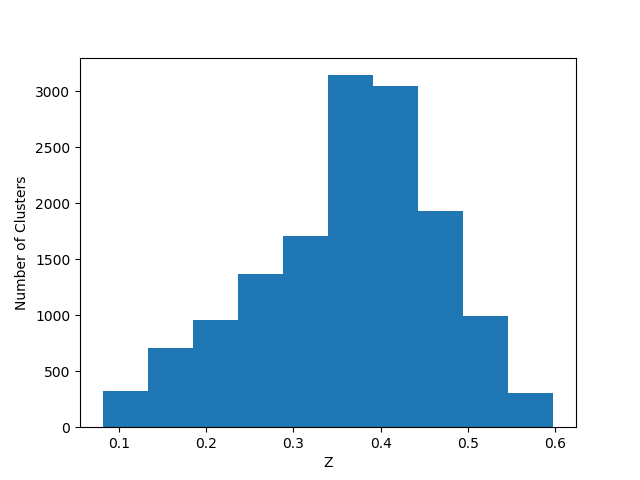
\includegraphics[width=0.5\textwidth]{../redmapper z hist.png}
\caption{This plot shows a histogram of the distribution of redshifts of the clusters in the RedMaPPer catalog. Evidently, the clusters in the RedMaPPer catalog range from $z\approx0.05$ to $z\approx0.6$. Note that this plot only includes clusters from RedMaPPer that were used in our analysis and thus does not include clusters that fell outside the range of our maps or were too close to point sources. }
\label{RedMaPPer Redshift Distribution}
\end{figure}

\begin{figure}[h]
\centering
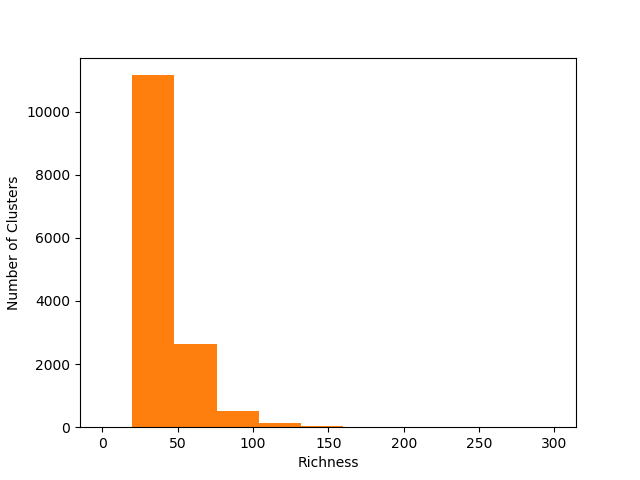
\includegraphics[width=0.5\textwidth]{../redmapper richness hist.png}
\caption{This plot shows a histogram of the distribution of the richnesses of the clusters in the RedMaPPer catalog. Evidently, the vast majority of clusters in the RedMaPPer catalog fall between richnesses of 25 and 100. Note that this plot only includes clusters from RedMaPPer that were used in our analysis and thus does not include clusters that fell outside the range of our maps or were too close to point sources. }
\label{RedMaPPer Richness Distribution}
\end{figure}

 \chapter{Theory and Methods}
\section{The tSZ Effect}
The tSZ effect is the result of inverse Compton scattering of photons from the CMB off of high energy electrons in hot gas. When CMB photons go through hot cluster gas they gain energy from the high energy electrons. Then when we measure the CMB these photons produce a frequency-dependent change in the observed CMB temperature along the Line-of-Sight (LOS) to the galaxy cluster (Greco et al.). The tSZ effect is quantified by the Compton-y parameter. The observationally relevant Compton-y parameter is the Comptonization parameter integrated along the full LOS within some aperture radius,
\begin{equation}
Y^{cyl}_{c}=d^{-2}_A(z) \frac{\sigma_T}{m_e c^2}\int_0^{R_c} 2 \pi R dR \int_{-\inf}^{\inf} dl P_e(r,M,z)
\end{equation}
Where $Y^{cyl}_{c}$ is the observed Compton-y parameter, $d_A(z)$ is the angular diameter distance to the cluster,$\sigma_T$ is the Thomson scattering cross-section, $m_e c^2$ is the rest mass of the electron, R is the  projected radius which we integrate up to $R_c$,  and $P_e(r,M,z)$ is the electron pressure profile (Greco et al.).
\section{Aperture Photometry}
To extract the Compton-y parameter from the CMB maps and differentiate it from effects of the dust and kSZ, we perform aperture photometry on the CMB maps at the locations of clusters indicated by the cluster catalogs. To perform aperture photometry we define a circular aperture of some radius (which we determined empirically to correspond to the typical radius of the tSZ effect at each frequency) surrounded by an annulus. We then subtract the mean pixel value in the annulus from the circular aperture and define the observed signal, $S_i$, to be the sum of the pixel values inside the circular aperture after this subtraction. The mean value of the annulus is subtracted to correct for large-scale foreground contamination, assuming it is roughly constant over the extracted aperture (Greco et al.). This signal, $S_i$, is then modeled just as described in Greco et al.,
\begin{equation}
\begin{aligned}
S_i=a_i Y^{cyl}_{c}+b_i D_c +\delta T_{CMB} \\
a_i=g(\nu_i) T_{CMB}\\
b_i=\left(\frac{\nu_i(1+z)}{\nu_0}\right)^\beta B (v_i(1+z),T_{dust})\left[\frac{\partial B(\nu_i,T)}{\partial T} \right]^{-1}_{T_{CMB}},
\end{aligned}
\end{equation}


where $g(\nu_i)=h\nu_i/k_B T_{CMB} coth(h\nu_i/2k_B T_{CMB})$, $T_{CMB}=2.7255 K$, $D_c$ is the amplitude of the dust emission integrated along the full LOS within the aperture radius, $v_0=353$ GHz is the reference frequency, $\beta=1.78$ is the dust spectral emissivity index, $T_{dust}= 20 K$ is the dust temperature, $B(\nu_i,T)$ is the Planck function, and $\delta T_{CMB}$ provides a constraint on bulk kSZ.\par
We do a weighted sum of the aperture photometry values for all the clusters at each frequency in which the weight of each value is inversely proportional to the amount of noise in that area of the map. Then we fit these weighted sums to the model above using emcee.
\begin{figure}[h]
\centering
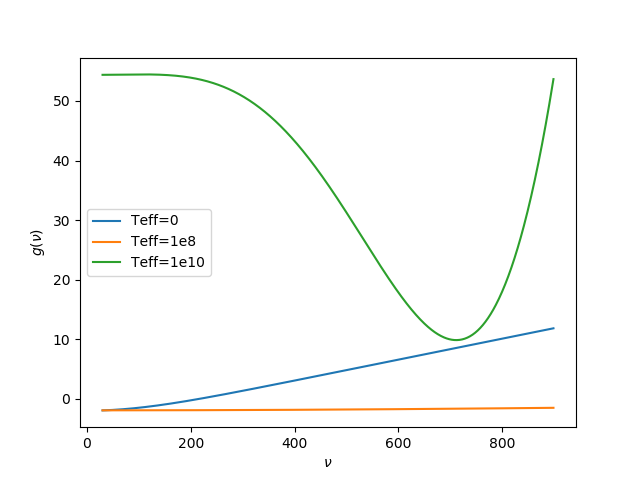
\includegraphics[width=0.5\textwidth]{../gnu.png}
\caption{This plot shows $g(\nu)$ as a function of frequency. }
%\label{$g(\nu)$}
\end{figure}

\begin{figure}[h]
\centering
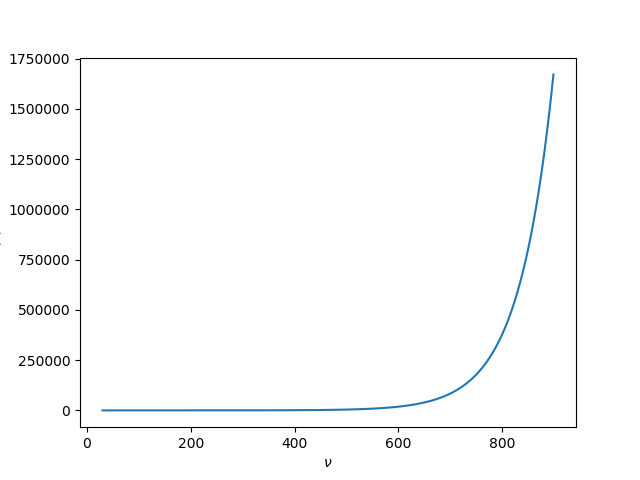
\includegraphics[width=0.5\textwidth]{../bdust.png}
\caption{This plot shows the dust coefficient as a function of frequency at a constant value of z=0.36315244, which is the average z value for our sample of galaxy clusters.}
%\label{$g(\nu)$}
\end{figure}


\section{Stacking}
In addition to doing this aperture photometry, we also use rectangular cutouts of the maps centered on the clusters as the to create unweighted and weighted stacks. These stacks provide a visual representation of the SZ effect at the different frequencies. Additionally ,the mean of the aperture photometry values of all the clusters at a given frequency should be the same as the aperture photometry values of the corresponding stacks. Thus, we were able to use the stacks to confirm our aperture photometry methodology. 
\chapter{Results}
Before doing the mcmc fitting, we performed a linear fit to the data by minimizing chi-squared. Here we only fit for two parameters, the Compton-y parameter and the integrated amplitude of the dust emission. Using this fit we found that $Y^{cyl}_{c}=7.96871772*10^{-17}$ and $D_c=5.74833793*10^{-18}$. This fit is plotted in the figure below.
\begin{figure}[h]
\centering
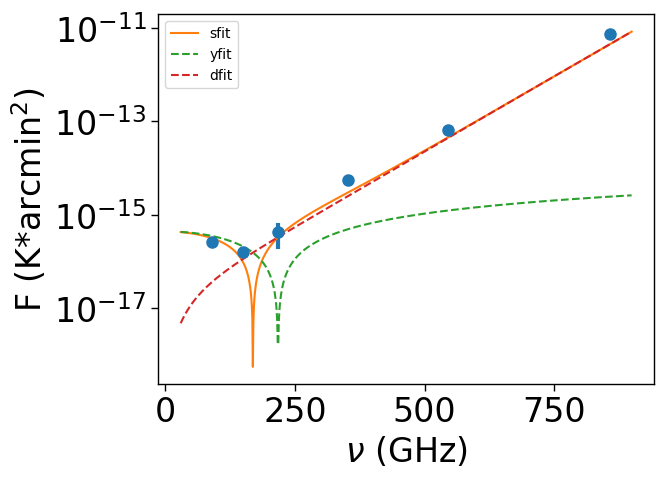
\includegraphics[width=0.5\textwidth]{../redmapper_apfluxes_fitlog.png}
\caption{This plot shows a linear fit of the data using only two fit parameters: Y (i.e. the Compton-y parameter) and D (the dust parameter). Note that the y-axis is on a log scale.}
%\label{$g(\nu)$}
\end{figure}

\chapter{Discussion and Conclusion}

\chapter{Future Research}

\chapter{References}
J. P. Greco, J. C. Hill, D. N. Spergel, and N. Battaglia,
Astrophys. J. 808, 151 (2015).
\end{document}
